\documentclass[a4paper,11pt]{article}
\usepackage[utf8]{inputenc}
\usepackage{xcolor}
\usepackage{amsmath}
\usepackage{amssymb}
\usepackage{tikz}
\usetikzlibrary{patterns}

\begin{document}

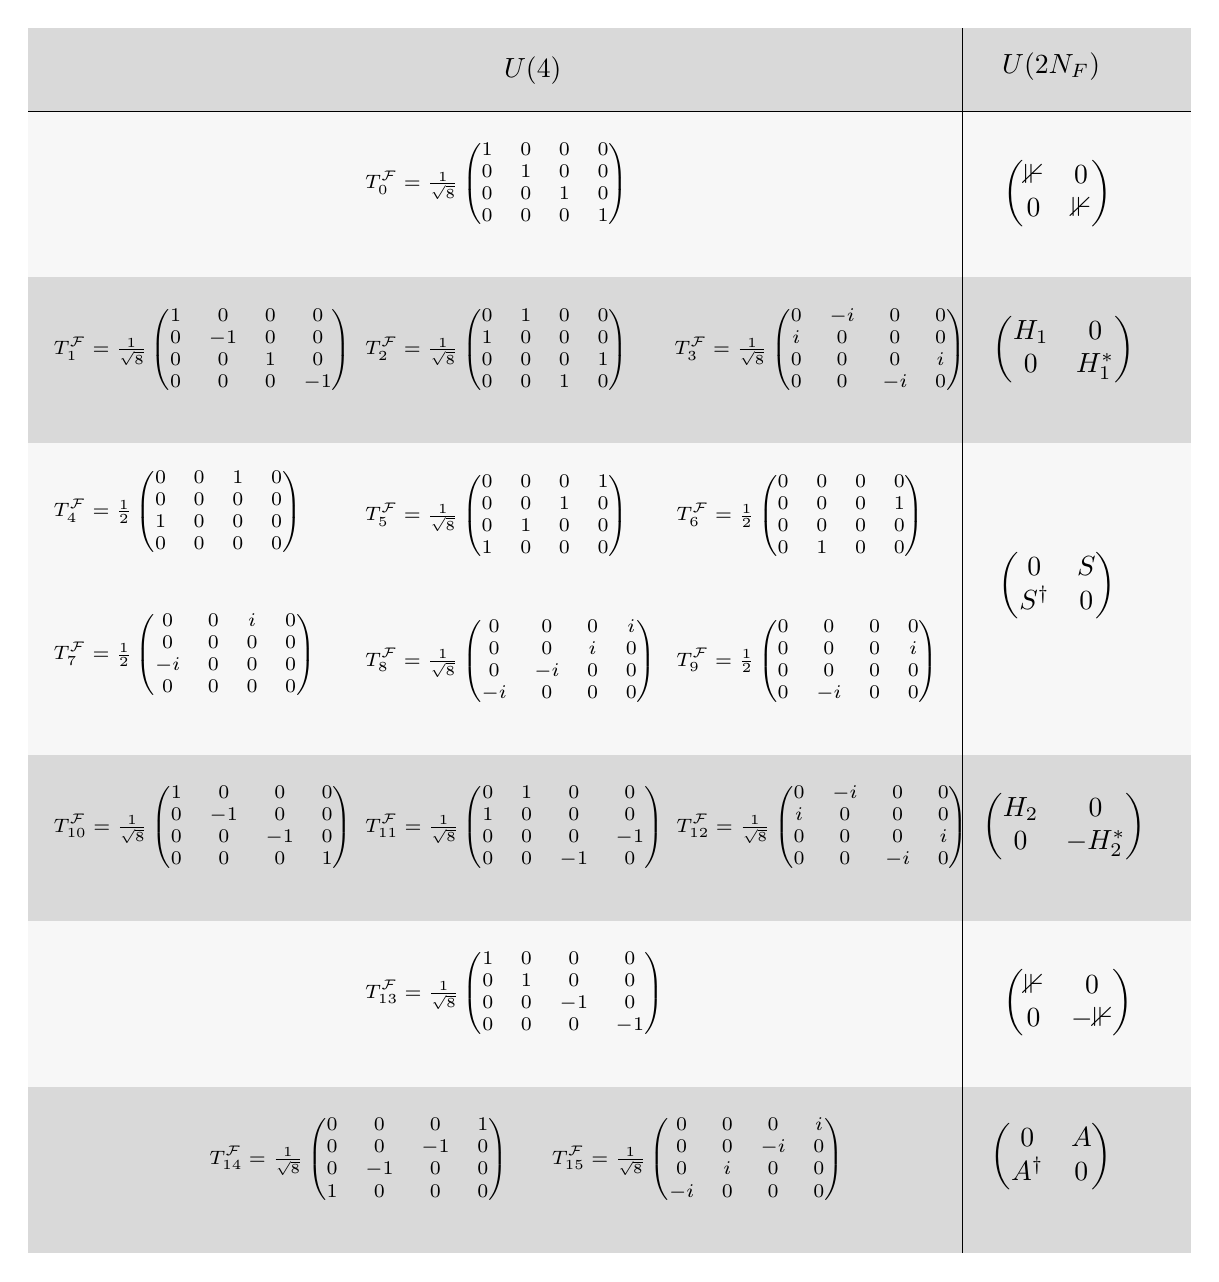
\begin{tikzpicture}[x=0.75pt,y=0.75pt,yscale=-1,xscale=1]

\draw  [draw opacity=0][fill={rgb, 255:red, 247; green, 247; blue, 247 }  ,fill opacity=1 ] (0,40) -- (560,40) -- (560,120) -- (0,120) -- cycle ;
\draw  [draw opacity=0][fill={rgb, 255:red, 217; green, 217; blue, 217 }  ,fill opacity=1 ] (0,120) -- (560,120) -- (560,200) -- (0,200) -- cycle ;
\draw  [draw opacity=0][fill={rgb, 255:red, 247; green, 247; blue, 247 }  ,fill opacity=1 ] (0,200) -- (560,200) -- (560,350) -- (0,350) -- cycle ;
\draw  [draw opacity=0][fill={rgb, 255:red, 217; green, 217; blue, 217 }  ,fill opacity=1 ] (0,350) -- (560,350) -- (560,430) -- (0,430) -- cycle ;
\draw  [draw opacity=0][fill={rgb, 255:red, 247; green, 247; blue, 247 }  ,fill opacity=1 ] (0,430) -- (560,430) -- (560,510) -- (0,510) -- cycle ;
\draw  [draw opacity=0][fill={rgb, 255:red, 217; green, 217; blue, 217 }  ,fill opacity=1 ] (0,510) -- (560,510) -- (560,590) -- (0,590) -- cycle ;
\draw  [draw opacity=0][fill={rgb, 255:red, 217; green, 217; blue, 217 }  ,fill opacity=1 ] (0,0) -- (560,0) -- (560,40) -- (0,40) -- cycle ;
\draw    (450,0) -- (450,590) ;
\draw    (0,40) -- (560,40) ;


% Text Node
\draw (161,132.4) node [anchor=north west][inner sep=0.75pt]  [font=\scriptsize]  {$T_{2}^{\mathcal{F}} =\frac{1}{\sqrt{8}}\begin{pmatrix}
0 & 1 & 0 & 0\\
1 & 0 & 0 & 0\\
0 & 0 & 0 & 1\\
0 & 0 & 1 & 0
\end{pmatrix}$};
% Text Node
\draw (11,132.4) node [anchor=north west][inner sep=0.75pt]  [font=\scriptsize]  {$T_{1}^{\mathcal{F}} =\frac{1}{\sqrt{8}}\begin{pmatrix}
1 & 0 & 0 & 0\\
0 & -1 & 0 & 0\\
0 & 0 & 1 & 0\\
0 & 0 & 0 & -1
\end{pmatrix}$};
% Text Node
\draw (310,132.4) node [anchor=north west][inner sep=0.75pt]  [font=\scriptsize]  {$T_{3}^{\mathcal{F}} =\frac{1}{\sqrt{8}}\begin{pmatrix}
0 & -i & 0 & 0\\
i & 0 & 0 & 0\\
0 & 0 & 0 & i\\
0 & 0 & -i & 0
\end{pmatrix}$};
% Text Node
\draw (11,210.4) node [anchor=north west][inner sep=0.75pt]  [font=\scriptsize]  {$T_{4}^{\mathcal{F}} =\frac{1}{2}\begin{pmatrix}
0 & 0 & 1 & 0\\
0 & 0 & 0 & 0\\
1 & 0 & 0 & 0\\
0 & 0 & 0 & 0
\end{pmatrix}$};
% Text Node
\draw (161,212.4) node [anchor=north west][inner sep=0.75pt]  [font=\scriptsize]  {$T_{5}^{\mathcal{F}} =\frac{1}{\sqrt{8}}\begin{pmatrix}
0 & 0 & 0 & 1\\
0 & 0 & 1 & 0\\
0 & 1 & 0 & 0\\
1 & 0 & 0 & 0
\end{pmatrix}$};
% Text Node
\draw (311,212.4) node [anchor=north west][inner sep=0.75pt]  [font=\scriptsize]  {$T_{6}^{\mathcal{F}} =\frac{1}{2}\begin{pmatrix}
0 & 0 & 0 & 0\\
0 & 0 & 0 & 1\\
0 & 0 & 0 & 0\\
0 & 1 & 0 & 0
\end{pmatrix}$};
% Text Node
\draw (11,279.4) node [anchor=north west][inner sep=0.75pt]  [font=\scriptsize]  {$T_{7}^{\mathcal{F}} =\frac{1}{2}\begin{pmatrix}
0 & 0 & i & 0\\
0 & 0 & 0 & 0\\
-i & 0 & 0 & 0\\
0 & 0 & 0 & 0
\end{pmatrix}$};
% Text Node
\draw (161,282.4) node [anchor=north west][inner sep=0.75pt]  [font=\scriptsize]  {$T_{8}^{\mathcal{F}} =\frac{1}{\sqrt{8}}\begin{pmatrix}
0 & 0 & 0 & i\\
0 & 0 & i & 0\\
0 & -i & 0 & 0\\
-i & 0 & 0 & 0
\end{pmatrix}$};
% Text Node
\draw (311,282.4) node [anchor=north west][inner sep=0.75pt]  [font=\scriptsize]  {$T_{9}^{\mathcal{F}} =\frac{1}{2}\begin{pmatrix}
0 & 0 & 0 & 0\\
0 & 0 & 0 & i\\
0 & 0 & 0 & 0\\
0 & -i & 0 & 0
\end{pmatrix}$};
% Text Node
\draw (161,442.4) node [anchor=north west][inner sep=0.75pt]  [font=\scriptsize]  {$T_{13}^{\mathcal{F}} =\frac{1}{\sqrt{8}}\begin{pmatrix}
1 & 0 & 0 & 0\\
0 & 1 & 0 & 0\\
0 & 0 & -1 & 0\\
0 & 0 & 0 & -1
\end{pmatrix}$};
% Text Node
\draw (86,522.4) node [anchor=north west][inner sep=0.75pt]  [font=\scriptsize]  {$T_{14}^{\mathcal{F}} =\frac{1}{\sqrt{8}}\begin{pmatrix}
0 & 0 & 0 & 1\\
0 & 0 & -1 & 0\\
0 & -1 & 0 & 0\\
1 & 0 & 0 & 0
\end{pmatrix}$};
% Text Node
\draw (251,522.4) node [anchor=north west][inner sep=0.75pt]  [font=\scriptsize]  {$T_{15}^{\mathcal{F}} =\frac{1}{\sqrt{8}}\begin{pmatrix}
0 & 0 & 0 & i\\
0 & 0 & -i & 0\\
0 & i & 0 & 0\\
-i & 0 & 0 & 0
\end{pmatrix}$};
% Text Node
\draw (11,362.4) node [anchor=north west][inner sep=0.75pt]  [font=\scriptsize]  {$T_{10}^{\mathcal{F}} =\frac{1}{\sqrt{8}}\begin{pmatrix}
1 & 0 & 0 & 0\\
0 & -1 & 0 & 0\\
0 & 0 & -1 & 0\\
0 & 0 & 0 & 1
\end{pmatrix}$};
% Text Node
\draw (161,362.4) node [anchor=north west][inner sep=0.75pt]  [font=\scriptsize]  {$T_{11}^{\mathcal{F}} =\frac{1}{\sqrt{8}}\begin{pmatrix}
0 & 1 & 0 & 0\\
1 & 0 & 0 & 0\\
0 & 0 & 0 & -1\\
0 & 0 & -1 & 0
\end{pmatrix}$};
% Text Node
\draw (311,362.4) node [anchor=north west][inner sep=0.75pt]  [font=\scriptsize]  {$T_{12}^{\mathcal{F}} =\frac{1}{\sqrt{8}}\begin{pmatrix}
0 & -i & 0 & 0\\
i & 0 & 0 & 0\\
0 & 0 & 0 & i\\
0 & 0 & -i & 0
\end{pmatrix}$};
% Text Node
\draw (459,137.4) node [anchor=north west][inner sep=0.75pt]  [font=\normalsize]  {$\ \begin{pmatrix}
H_{1} & 0\\
0 & H_{1}^{*}
\end{pmatrix}$};
% Text Node
\draw (462,251.4) node [anchor=north west][inner sep=0.75pt]  [font=\normalsize]  {$\ \begin{pmatrix}
0 & S\\
S^{\dagger } & 0
\end{pmatrix}$};
% Text Node
\draw (458,526.4) node [anchor=north west][inner sep=0.75pt]  [font=\normalsize]  {$\ \begin{pmatrix}
0 & A\\
A^{\dagger } & 0
\end{pmatrix}$};
% Text Node
\draw (464,452.4) node [anchor=north west][inner sep=0.75pt]  [font=\normalsize]  {$\ \begin{pmatrix}
\mathbb{1} & 0\\
0 & -\mathbb{1}
\end{pmatrix}$};
% Text Node
\draw (454,367.4) node [anchor=north west][inner sep=0.75pt]  [font=\normalsize]  {$\ \begin{pmatrix}
H_{2} & 0\\
0 & -H_{2}^{*}
\end{pmatrix}$};
% Text Node
\draw (228,12.4) node [anchor=north west][inner sep=0.75pt]    {$U( 4)$};
% Text Node
\draw (468,10.4) node [anchor=north west][inner sep=0.75pt]    {$U( 2N_{F})$};
% Text Node
\draw (161,52.4) node [anchor=north west][inner sep=0.75pt]  [font=\scriptsize]  {$T_{0}^{\mathcal{F}} =\frac{1}{\sqrt{8}}\begin{pmatrix}
1 & 0 & 0 & 0\\
0 & 1 & 0 & 0\\
0 & 0 & 1 & 0\\
0 & 0 & 0 & 1
\end{pmatrix}$};
% Text Node
\draw (464,62.4) node [anchor=north west][inner sep=0.75pt]  [font=\normalsize]  {$\ \begin{pmatrix}
\mathbb{1} & 0\\
0 & \mathbb{1}
\end{pmatrix}$};


\end{tikzpicture}

\end{document}